\documentclass[usenatbib]{mnras}

% Packages needed
\usepackage{newtxtext,newtxmath}  % Times-like font (MNRAS requirement)
\usepackage[T1]{fontenc}          % Required for MNRAS
\usepackage{graphicx}             % Figures
\usepackage{amsmath, amssymb}     % Mathematics support
\usepackage{natbib}

% Title
\title[Shape of Merger Remnant]{The Morphology of the MW-M31 Merger Remnant: Ending Shape}
% Author list
\author[Jessica Gurney]{
Jessica Gurney$^{1}$\thanks{E-mail: jgurney@arizona.edu}
\\
% List of institutions
$^{1}$University of Arizona, Astronomy Department\\
}
\date{April 11, 2025}

% Start the document
\begin{document}
\maketitle

\begin{keywords}
Major Merger -- Spiral Galaxy -- Elliptical Galaxy -- Triaxial -- Isodensity Contours
\end{keywords}


The \textbf{Stellar Disk} The first time a keyword appears in main text bold it
A \textbf{Major Merger} or define with equation

\section{Introduction}
Galaxies come in all shapes and sizes, from flat rotating disks with spiral arms to massive unstructured spheroids. One of the most dramatic drivers of galaxy shape evolution is a \textbf{Major Merger}, which is when two galaxies of similar mass collide into each other and form a new merged galaxy. The Andromeda galaxy (M31) and the Milky Way (MW) are two galaxies inside the \textbf{Local Group}. The Local group is a vast region of space where many galaxies, mostly dwarf galaxies, are gravitationally bound together. Both the Milky Way and Andromeda are classified as \textbf{Spiral Galaxies}, characterized by the flat rotating stellar disk, with distinct arms that twirl around the center. Simulations predict that these two galaxies will merge in the next several billion years, forming a single, more massive remnant called an \textbf{Elliptical Galaxy}. Elliptical galaxies show less structure than spiral galaxies, and the stars orbit in random paths creating shapes that look like ovals or spheres. The MW-M31 merger is a unique opportunity to study the internal structure of an Elliptical galaxy once it reaches an equilibrium point, specifically if its shape and classification vary with radius. One method of assessing this transformation is looking at the stellar density via \textbf{Isodensity Contours}, which are lines on a map that mark off regions of equal density. Isodensity contours allow us to visualize the spatial distribution of structures so that we can infer whether the galaxy is spherical, oblong, or triaxal, and if these shapes are consistent at different radii. 

A \textbf{galaxy}, as defined by \cite{willman2012}, is a gravitationally bound collection of stars whose properties cannot be explained by a combination of baryons (gas, dust, and stars) and Newton’s laws of gravity. \textbf{Galaxy Evolution} refers to how galaxies and their components develop over cosmic time. These transformations include internal mechanisms like star formation and external gravity interactions like mergers, accretion, and tidal stripping. Studying major mergers is critical in recognizing the evolution of a galaxies life, which lead us to understand the history of our universe based on galaxies we can observe. The MW-M31 system is useful for this because we can study the detailed evolution of two spiral galaxies undergoing a major merger, including how mass, angular momentum, and morphology evolve during and after the collision. 

Research has shown that the main ways elliptical galaxies form are from major mergers between spiral galaxies. \cite{barnes92} showed through simulation that when two disk galaxies merge in a roughly head on orbit a violent randomization of orbits happen, which results in an elliptical or spheroidal system. The final morphology depends on several factors; mass ratios, starting orbital angular momentum, dust content, dark matter mass, and the presence of a pre-existing bulge. It is important to note that galaxies in the process of merging are irregular, as illustrated in Figure~\ref{fig:morphology}. Isodensity mapping is essential to understanding how merged galaxies settle, and allow us to classify the final morphology shape. 

\begin{figure}[h]
    \centering
    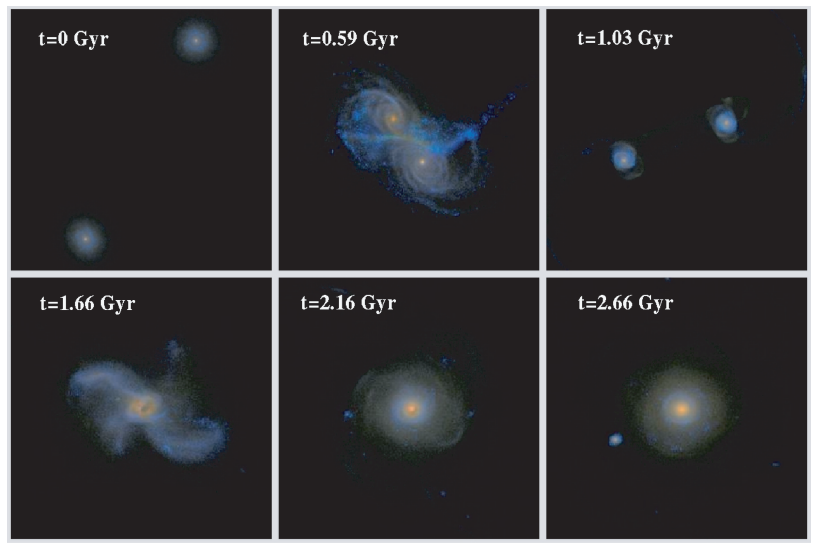
\includegraphics[width=0.4\textwidth]{Galaxy_Merger_J.M.Lotz.png}
    \caption{Evolution of simulation of a major galaxy merger. The time displayed in each image is the evolution of the system from the start of the simulation. The top row shows the pre-merger galaxies with a pass by, and the bottom row shows when the merger forms a nuclei and settles into the final remnant form. The field of view for t=0 \& t=1.03 Gyr is 200 kpc, while the rest are 100 kpc. The blue represents star forming regions, tidal tails, and outer regions. Red represents dust-enshrouded star-forming nuclei. \citet{lotz08}.}
    \label{fig:morphology}
\end{figure}

There are many questions in our understanding of galaxy formation through mergers. A key one is whether the merger remnant will relax into a sphere, or if it retains elongations that reflect pieces of the previous galaxy? \citet[p. 724-725]{barnes92} ran N-body simulations and found that disk galaxies only form elliptical cores if the galaxies have pre-existing bulges and if they were head on collisions, while inclined encounters create flattened remnants. Another question is if we can see structures from the individual galaxies, do those structures appear throughout the full galaxy, or does proximity to the center of the merger affect that? The findings in \citet[p. 13]{vandermarel12b} saw the inner regions of a remnant looked spherical, while the outer contours had features of previous galaxies such as the shell and tails. The third question is how does the gas content, Wet (gas-rich) or Dry (gas-poor), of a galaxy influence the final structure of the merger? While comparing wet and dry merger simulations,\citep[p. 12]{lin10} found that dry mergers produced boxy and slow rotating galaxies, hinting that wet mergers appear different, suggesting that gas can be behind the final shape of a merger remnant.  

\section{Proposal}

\subsection{This Project}
In this project I will study the final morphology of the remnant formed by the MW and M31 galaxy merger. Specifically, I will determine if the resulting system is elongated or a perfect sphere using the Hubble classification of Ellipses (E0-E7). A key focus will be if the shape changes based on radius, which can reveal whether structural changes are radius-dependent. For that, I will plot iso-density contours on a post-merger snapshop from an N-body simulation. This will involve generating density maps of the 3 planes (face-on, side-view, top-view), fitting ellipses to the iso-density contours, and assigning the classification number (E0-E7) to the contours at different radii. I can then quantify how the contours on each plane change per radii. 

This project directly addresses the question of whether MW-M31 remnant varies with radius, and whether the inner and outer regions have varying degrees of relaxation. Simulations such as those by \citet[PDF p. 16]{vandermarel12b} have shown that even 10 Gyr after merger, outer regions may retain shells or asymmetries while inner regions appear more relaxed. This implies remnant may appear differently depending on the scale and depth of observation. My project looks into this by measuring how the axis ratio and ellipticiy of the iso-density contours change with radius, which will determine if a single Hubble classification is enough to describe the entire remnant. 

Understanding how merger remnants settle, whether its into a fully relaxed spheroid, or preserving pieces of old galaxies with elongation, is important in the study of Galaxy Evolution. Major mergers are thought to be the dominant way in transforming spiral galaxies into spherical galaxies. However, if structural abnormalities are found at specific radii, then the assumption that all mergers end up as spherical galaxies may be over simplified. By studying the radial variation in shape and elongation, this project may impact how we classify galaxy morphology, especially if cases such as viewing angle affects the classification. It also can show how long merger signatures persist, which is critical in reconstructing merger histories in our universe. 

\subsection{Methods}

This project uses the \citet{vandermarel12a,vandermarel12b} MW-M31 merger simulation to analyze the final stellar morphology of the merger remnant. The simulation was conducted with an N-body simulation, where in each mass element (particles representing a stellar star) undergo gravity interactions with the other particles over time. Each galaxy is modeled with a combination of a dark matter halo, a stellar disk, and central bulge. For this simulation I focused on the stellar components in the galaxies, particles of the disk (type 2) and the bulge (type 3), this was to isolate the observable galaxy. 

The simulation uses the high-resolution MW and M31 dataset. A comparison between snapshots 5-7 Gyr (snapshot 500, 600, 700), was chosen because this was after the galaxies had merged and relaxed. Using my own Python implementation, I first merge the stellar particles from both galaxies into a single data file. Next, I compute the total mass-weighted center of mass (COM) position and velocity using \texttt{CenterofMass.py}, of the bulk and disk particles. The analysis is carried out in units of kiloparsecs and km/s.

After centering the system, I compute the angular momentum vector of the remnant using:
\[
\mathbf{L} = \sum_i m_i (\mathbf{r}_i \times \mathbf{v}_i)
\]
where \( m_i \) is the mass of particle \( i \), \( \mathbf{r}_i \) is its position relative to the center of mass, and \( \mathbf{v}_i \) is its velocity. To orient the galaxy for a face on view I find the angular momentum vector and see how much it angles from the Z-axis. A skew-symmetric matrix is constructed \( \mathbf{K} \) from the rotation axis and apply the rotation matrix:
\[
\mathbf{R} = \mathbf{I} + \mathbf{K} + \mathbf{K}^2 \cdot \left(\frac{1 - \cos\theta}{\sin^2\theta}\right)
\]
where \( \mathbf{I} \) is the identity matrix and \( \theta \) is the angle between \( \hat{\mathbf{L}} \) and \( \hat{\mathbf{z}} \). This realigns all particle positions and velocities so that the disk lies in the XY plane.


\begin{figure}
    \centering
    \includegraphics[width=0.45\textwidth]{XY_600.png}
    \caption{Methodological overview. After centering and rotating the merger remnant, I compute the 2D surface density in three planes (XY, XZ, YZ), extract isodensity contours, and fit ellipses to each level. Shown is the XY Plane or Face-on View of the remnant at 600 Gyrs.}
    \label{fig:flowchart}
\end{figure}

The surface density is computed in each 2D plane using a weighted histogram of particle positions:
\[
\Sigma(R) = \frac{\sum m_i}{A}
\]
where \( m_i \) are the masses of the particles within each bin of area \( A \), and \( \Sigma(R) \) is the resulting surface density. First I construct the iso-density contour over the density maps corresponding to fixed confidence levels (e.g., 40\%, 65\%, 90\%, 99\%), the contours as smoothed with a gaussian function to eliminate small fluctuations in shape. Each contour is then fit with an ellipse using \texttt{EllipseModel()} from \texttt{skimage.measure}, and the axis ratio is computed for each level:
\[
\frac{b}{a}
\]

The Hubble E-type classification (E0-E7) is then assigned to each contour based on:

\[
E = \text{int}(10 \times (1 - b/a))
\]

It is then time to see if the remnant is spherical, elongated, or traixial and how this varies with radius. I generate three plots:

\begin{itemize}
    \item \textbf{2D Surface Density Maps (XY, XZ, YZ):}  
    These face-on, top-down, and side-view projections show the distribution of stellar mass. By visually comparing the shape of the remnant in all three planes, I can identify signs of elongation, flattening, or any other types of distortions that deviate from a spherical shape. 

    \item \textbf{Isodensity Contours with Ellipse Overlays:}  
    Isodensity contours show enclosed density where a certain percentage of stellar mass resides, e.i. contour 60 is where 60\% of the galaxy resides in. These contours allow me to see how the shape changes at different radii, since each confidence level ends up being at its own distance. Circular contours indicate spheroidal symmetry, while elongated ellipses suggest triaxiality.

    \item \textbf{Grouped Bar Chart of \( b/a \) vs Radius with E-Types:}  
    This summary plot visualizes how the axis ratio \( b/a \), which is a direct measurement of flattening, varies with radius in each projection. By using these axis ratios to find the Hubble E-types at each contour, I can see if the galaxy has a consistent morphological class throughout or if it changes with increasing radius. This plot answers the core question of my project: does the remnant exhibit different structural classifications at different radii?
\end{itemize}

\section{Results}

\subsection{Projected Density and Ellipse Fits at 700 Gyr}

Figure~\ref{fig:contours} shows the projected 2D surface density of the merger remnant at 700 Gyr in the XY (face-on), XZ (top-down), and YZ (side) planes. For each plane, the left panels show the smoothed surface density with confidence level contours which encapsulates a total percentage of the galaxy. The confidence levels shown are 10\% 45\%, 80\%, 90\%, 95\%, 99\% which were chosen because the majority of the radii increased ~10 kpc. This allows us to compare the symmetry and of the remnant as a function of radius. The right panels show ellipses fitted to those contours using a custom function that finds the largest contour and fits an ellipse to it. The ellipse function contains information such as ellipse origin, major (a) and semi major (b) axes sizes, etc. These two graphs allow us to see the overall shape of the galaxy at different radii. In the left we can see more of the natural shape of the remnant; the center has fairly smooth contours that become stretched and wobbly the farther we move out. In the right this is mimicked with the fitted ellipses with fairly circular centers that elongate at large radii. We have another step of comparison by places all 3 planes next to each other to give us a view of the 3D remnant. A perfectly spherical remnant would have the same shape in all 3 planes, but we see that from different views the remnant will appear more spherical from one direction (XY), and stretched in the others.  

\begin{figure*}
    \centering
    \includegraphics[width=\textwidth]{XY_700.png}
    \includegraphics[width=\textwidth]{XZ_700.png}
    \includegraphics[width=\textwidth]{YZ_700.png}
    \caption{
    \textbf{Surface Density and Ellipse Fits for the Remnant at 700 Gyr.}
    Each row shows a 2D projection of the system: XY (top), XZ (middle), and YZ (bottom). 
    Left: Smoothed surface density maps with overlaid confidence-level contours, where the colorbar shows $\log_{10}$(surface density).
    Right: Ellipses fitted to the contours from the left panel, color-coded by contour level.
    Axis labels are in kpc. 
    \textit The remnant becomes increasingly elongated with radius.
    }
    \label{fig:contours}
\end{figure*}


\subsection{Axis Ratio Evolution from 600 to 700 Gyr}

Figure~\ref{fig:barplot} compares the axis ratios $b/a$ of ellipses fitted at the various average radii for two different times: 600 Gyr and 700 Gyr. This was generated using a custom grouped bar plot function that displays the XY, XZ, and YZ projections side by side, and each bar labeled by its corresponding ellipse E-type (E0–E7). The central region of the remnant are highly spherical in all projects with their classifications around E1. At larger radii the ellipses become more elongated falling into the E2/E3 range. Across the planes we see at close radii the planes are very similar, but as we go out the difference in the plane becomes random, sometimes very close in shape, or very different. When we look at the structure of the 700 Gyr plot the trends stay the same. However when we compare 600 and 700 Gyr, the 700 Gyr has the bars at each radii at a higher ($b/a$) ratio than the 600 Gyr plot. This suggests while the inner regions remain near-spherical (E0–E1), the remnant develops greater elongation in its outer parts, while relaxing into a spherical shape over time. 

\begin{figure*}
    \centering
    \includegraphics[width=0.48\textwidth]{Bar_600.png}
    \includegraphics[width=0.48\textwidth]{Bar_700.png}
    \caption{
    \textbf{Axis Ratio $b/a$ vs. Radius for 600 Gyr (left) and 700 Gyr (right).}
    Each bar represents the axis ratio of a fitted ellipse in a given projection plane: XY (gold), XZ (pink), and YZ (purple). 
    Bars are grouped by average radius (x-axis), and labeled by E-type classification (E0–E7) based on $b/a$ values.
    Outer contours in the YZ plane show increasing elongation over time, reflecting gradual evolution in the vertical structure of the remnant.
    }
    \label{fig:barplot}
\end{figure*}

\section{Discussion}

One of the key results from the previous section is the trend in axis ratio ($b/a$) with radius and projection plane. At 700 Gyr, the remnant appears nearly spherical in the central regions across all planes (E1), but becomes progressively elongated (E2–E3) in the outer regions. The pattern was consistent with my hypothesis that suggests the interior stars lose memory of their original disk configuration due to gravitation chaos during the merger, while stars in the outer halo may be able to preserve some pre-merger structures.

My result is consistent with previous literature on galaxy mergers. For example, \citet{Barnes1992} and \citet{Hopkins2008} show that violent interactions during major mergers redistribute stellar orbits, leading to a bulged or spheroid central structure. The outer regions are less affected by gravitational interactions and may retain tidal features, shells, or remnants of spiral arms (\citealt{Duc2013}). The significance of this result is that it supports the idea that the morphology of a merger has radius-dependent features. Outer structures of ellipses can retain clues about a galaxies pre-merger identity, and that those features can become less prominent over time. This can give us a new way to estimate ages of galaxies and give us clues about the galaxies pre-merger identities. 


There are, however, several uncertainties in this analysis. Most importantly, the simulation does not include dark matter particles. Since dark matter dominates the total mass and gravitational potential at large radii, its absence may lead to underestimating the stability or shape of the outer regions. Additionally, I do not account for gas or dust regions which could create a region of star formation during or after the merger. New stars could introduce additional gravitation interactions, furhter changing the remnants morphology over time. Lastly, by choosing a large snapshot spacing (600 to 700 Gyr) I may be missing short-time scale variations or substructures that may appear due to the merger, and in fact what we may be see is not elongation from the previous galaxies structures. 

\section*{Acknowledgments}
Some of the code development was supported by OpenAI’s ChatGPT. Specifically, ChatGPT was used to help draft Python functions for merging the snapshot data into a single file, generating the fitted ellipses over the contours, and creating a grouped bar plot of axis ratios. All code was then reviewed, tested, and edited.
ChatGPT also helped format this document into MNRAS format, and gave minor editing critique on this report. All suggestions were reviewed for accuracy and authenticity before being accepted or rejected. 

\bibliographystyle{aasjournal}

\begin{thebibliography}{}
\bibitem[Barnes \& Hernquist(1992)]{barnes92} Barnes, J. E., \& Hernquist, L. E. 1992, ARA\&A, 30, 705
\bibitem[Eliche-Moral et al.(2018)]{eliche18} Eliche-Moral, M. C., et al. 2018, A\&A, 617, A113
\bibitem[Lin et al.(2010)]{lin10} Lin, L., Cooper, M. C., Jian, H.-Y., et al. 2010, ApJ, 718, 1158, doi:10.1088/0004-637X/718/2/1158
\bibitem[Lotz et al.(2008)]{lotz08} Lotz, J. M., et al. 2008, MNRAS, 391, 1137
\bibitem[Van der Marel et al.(2012a)]{vandermarel12a} van der Marel, R. P., Besla, G., et al. 2012, 753
\bibitem[Willman \& Strader(2012)]{willman2012}
Willman, B., \& Strader, J. 2012, AJ, 144, 76, doi:10.1088/0004-6256/144/3/76
\end{thebibliography}

 
\end{document}
